\documentclass[conference]{IEEEtran}

\usepackage{cite}
\usepackage{amsmath,amssymb,amsfonts}
\usepackage{algorithmic}
\usepackage{graphicx}
\usepackage{textcomp}
\usepackage{xcolor}
\usepackage[hidelinks]{hyperref}
\usepackage{booktabs}
\usepackage{array}
\usepackage{multirow}
\usepackage{url}

\def\BibTeX{{\rm B\kern-.05em{\sc i\kern-.025em b}\kern-.08em
    T\kern-.1667em\lower.7ex\hbox{E}\kern-.125emX}}

\begin{document}

\title{MicroBird: Microjoule-Range Embedded Bird-Call Classification\\for Irish Species Monitoring on the MAX78002}

\author{
\IEEEauthorblockN{Justyna Przyborska}
\IEEEauthorblockA{
\textit{Immersive Software Engineering} \\
\textit{University of Limerick} \\
Limerick, Ireland \\
23303816@studentmail.ul.ie
}
}

\maketitle

\begin{abstract}
This paper presents MicroBird, a complete end-to-end embedded bird-call classification system for Irish species monitoring on the MAX78002 AI microcontroller. The pipeline spans regional dataset curation from Xeno-Canto, clip-level teacher filtering using BirdNET, $64{\times}128$ log-mel spectrogram generation with per-sample normalisation, SpecAugment and Mixup data augmentation, and hardware-aware quantization-aware training (QAT). A systematic ablation study across ten architecture configurations examines the trade-off between channel width, network depth, residual connections, and post-quantization accuracy. The best-validated model achieves 83.01\% top-1 QAT validation accuracy across 51 classes (50 Irish species plus a non-bird background class); a 245,695-parameter configuration evaluated offline on the held-out test set reaches 80.59\% top-1 and 91.53\% top-3 accuracy. The deployed DW1 model (393,160 parameters, $\approx$384~KB) is synthesised for the MAX78002 and driven by a matching on-device C spectrogram pipeline, achieving 79.10\% top-1 and 90.90\% top-3 accuracy on a full 3{,}034-sample end-to-end hardware/API evaluation of the held-out test split. On-device measurement shows CNN inference completes in 3.5~ms consuming 15.3~\textmu J, with total pipeline energy of approximately 0.69~mJ per 3-second clip. Compared against published embedded bird classifiers, MicroBird achieves 61--4{,}000$\times$ lower energy per inference while sustaining high 51-class accuracy, demonstrating that dedicated CNN accelerators offer a qualitative efficiency advantage over general-purpose microcontroller deployment for wildlife acoustic monitoring.
\end{abstract}

\begin{IEEEkeywords}
MicroBird, embedded AI, bird-call classification, Irish wildlife monitoring, acoustic monitoring, MAX78002, quantization-aware training, TinyML
\end{IEEEkeywords}

% =================================================================
\section{Introduction}

\subsection{Motivation}
Monitoring bird populations provides valuable insight into biodiversity, habitat quality, and the ecological effects of climate change. Birds are widespread, comparatively well studied, and relatively easy to detect, which makes them effective indicator species for long-term environmental monitoring. Because many bird populations respond measurably to land-use change, habitat degradation, and warming temperatures, bird trends can act as an early warning system for wider ecosystem disruption. As a result, scalable bird monitoring has become an important task in conservation science.

Passive acoustic monitoring offers a practical way to observe bird presence over long periods without requiring continuous human fieldwork. However, while autonomous recording units make large-scale audio collection possible, turning those recordings into reliable species detections remains difficult and expensive when it depends on manual review. This creates a clear need for automated and low-cost bird-call classification systems that can operate efficiently in real deployment conditions.

\subsection{Problem Statement and Research Gap}
Recent advances in deep learning have significantly improved automated bird-call classification. Systems such as BirdNET demonstrate that convolutional models operating on spectrogram representations can achieve strong classification performance across large species sets. However, many current solutions still depend on cloud inference or relatively power-hungry edge hardware, which limits their practicality for wide deployment in remote monitoring scenarios.

This project focuses on a gap between high-capacity bird audio classifiers and the needs of low-cost, stationary regional monitoring systems. Many current classifiers are designed to identify hundreds or thousands of species in a single model, even though a fixed deployment site is likely to encounter only a much smaller regional subset. For a battery-powered embedded node, this broader class space increases computational cost, memory requirements, and model complexity without necessarily improving usefulness at the target location. A smaller region-specific model may therefore offer a better trade-off between practicality, efficiency, and classification performance.

\subsection{Project Objectives}
The primary objective of this project is to design, train, and deploy a low-power embedded bird-call classifier for Irish species monitoring on the MAX78002 platform. To achieve this, the project develops an end-to-end pipeline spanning regional species selection, public-audio dataset construction, clip-level teacher filtering, log-mel spectrogram generation, data augmentation, QAT model training, hardware synthesis, and on-device inference.

A key goal is not only to train an accurate classifier, but to produce a model and preprocessing workflow that remain compatible with the strict hardware constraints of the target device. This includes managing limited memory, quantized inference requirements, and the practical requirements of real-time audio classification from short clips. The wider aim is to explore whether compact embedded models can provide a feasible foundation for distributed wildlife monitoring systems in Ireland.

\subsection{Contributions of This Work}
This work makes the following contributions. First, it develops a curated region-specific bird-audio dataset pipeline tailored to Irish monitoring scenarios rather than global bird classification. Second, it introduces a clip-level label-cleaning stage using BirdNET as a teacher model to improve the quality of short training examples extracted from community recordings. Third, it implements a log-mel spectrogram preprocessing pipeline and hardware-aware training workflow, including a systematic ablation study over model width, depth, and residual connections. Fourth, it delivers a complete embedded deployment comprising hardware synthesis, on-device spectrogram computation in C, and a host-side API and web interface for live demonstration. Finally, it evaluates the system's energy profile and compares it against relevant baselines, quantifying the practical trade-off between accuracy and power consumption.

% =================================================================
\section{Background and Related Work}

\subsection{Bird Population Monitoring and Passive Acoustic Monitoring}
For many years, bird monitoring relied heavily on human-led field methods such as point counts, in which observers visually or aurally identify birds at fixed locations over timed intervals. While effective, these methods are labour-intensive and difficult to scale across large geographic areas or long monitoring periods. Passive acoustic monitoring has improved this situation by allowing autonomous devices to collect environmental audio over extended time spans. This provides richer temporal coverage and reduces the need for constant field presence.

Despite these advantages, passive acoustic monitoring generates very large audio datasets that are expensive to analyse manually. This has made automated classification increasingly important. The central challenge is therefore no longer only how to collect bird audio, but how to process it accurately, efficiently, and at scale.

\subsection{Bird-Call Classification from Audio}
Bird-call classification has evolved significantly over the last decade. Earlier systems often relied on handcrafted acoustic features combined with classical machine-learning models such as support vector machines, random forests, and decision trees. More recent approaches instead use time--frequency representations, particularly log-mel spectrograms, together with convolutional neural networks. This shift has enabled much stronger performance, especially on larger and more variable audio datasets.

Large modern systems such as BirdNET \cite{kahl2021birdnet} show the effectiveness of spectrogram-based deep learning for bird audio analysis. These systems are powerful, but they are typically designed for broad global classification tasks and often require substantial computational resources. Their success nevertheless establishes an important foundation for this project: bird vocalisations can be represented effectively as spectrogram images and classified using convolutional architectures.

\subsection{Edge AI for Biodiversity Monitoring}
Running inference closer to the data source has clear advantages for biodiversity monitoring. Edge inference can reduce bandwidth use, avoid continuous raw-audio transfer, improve privacy, and lower long-term storage costs. It also makes persistent monitoring more realistic in remote areas where network access may be limited or unreliable.

Some recent systems have therefore moved toward edge-based acoustic classification. However, many of these still rely on comparatively powerful embedded computers such as Jetson-class devices. While such platforms reduce cloud dependence, they remain relatively expensive, power-hungry, and difficult to scale into dense networks of low-maintenance wildlife sensors. This motivates the exploration of even smaller and lower-power AI hardware for fixed-site acoustic monitoring.

\subsection{Quantization-Aware Training for Embedded CNNs}
Deploying neural networks on microcontrollers requires reducing weight and activation precision to 8 bits or fewer. Post-training quantization (PTQ) calibrates fixed-point scale factors from a small dataset after training. Quantization-aware training (QAT) \cite{jacob2018quantization} improves over PTQ by simulating quantization noise during the training process itself, allowing weights to adapt and recover accuracy that PTQ would otherwise lose. For small models with fewer than one million parameters, QAT typically recovers 1--5 percentage points of accuracy relative to PTQ.

\subsection{Hardware Constraints of the MAX78002 Platform}
The MAX78002 is an ultra-low-power AI microcontroller with a dedicated CNN accelerator, making it an attractive platform for battery-powered edge inference \cite{adi2022training}. Unlike general-purpose computing hardware, it imposes strict constraints on deployable models. CNN weight SRAM is limited to 512~KB, supported operator types are restricted to fused convolution-activation primitives, and preprocessing must be implemented on the Cortex-M4 coprocessor. These constraints directly affect model architecture, input size, quantization strategy, and deployment flow. In this project, the MAX78002 is therefore not simply the final deployment target; it is a core design constraint that shapes the entire pipeline.

% =================================================================
\section{Methodology}

\subsection{Overall System Design}
The system is designed as a complete end-to-end pipeline. Audio recordings are downloaded from Xeno-Canto \cite{vellinga2015xc} and segmented into three-second clips, which are filtered using BirdNET \cite{kahl2021birdnet} as a teacher classifier. Accepted clips are converted to $64 \times 128$ log-mel spectrograms, normalised, and split into training, validation, and test sets. A hardware-aware CNN is trained using QAT and synthesised for the MAX78002 using the Analog Devices ai8x toolchain \cite{adi2022training}. On the device, a matching C spectrogram pipeline feeds the CNN accelerator for real-time inference, with results surfaced via a host-side API and web interface.

\begin{figure}[t]
\centering
% TODO: Upload your pipeline block diagram to Overleaf as "fig1_pipeline.pdf" (or .png)
% Create in draw.io: two-row flow from Xeno-Canto → manifest → filter → BirdNET teacher
% → spectrogram → QAT training → synthesis → MAX78002 → Flask API → Web UI
\includegraphics[width=\columnwidth]{fig1_pipeline.pdf}
\caption{End-to-end MicroBird pipeline. Top row: data collection and preprocessing ---
Xeno-Canto recordings are windowed, RMS-gated, and teacher-filtered by BirdNET to produce
labelled $64{\times}128$ log-mel spectrograms. Bottom row: model training and deployment ---
the QAT-trained CNN is synthesised for the MAX78002 and driven by a matching on-device
C spectrogram pipeline, with results exposed through a Flask API and web interface.}
\label{fig:pipeline}
\end{figure}

Two design decisions cut across all stages. First, the 51-class set (50 species plus a non-bird background class) was chosen to fit within the MAX78002's 512~KB CNN SRAM. Second, all preprocessing parameters were fixed early and applied identically in both the Python training pipeline and the C firmware, ensuring that training-time and deployment-time inputs are numerically consistent.

\subsection{Dataset Construction}

\subsubsection{Species Selection}
Species were selected to create a region-specific class set that matched the intended Irish fixed-site monitoring scenario while remaining feasible for low-power embedded deployment on the MAX78002.

To construct the species list, eBird reporting data was used to identify commonly observed bird species in Ireland, as it provides large-scale citizen-reported frequency information. This was then cross-referenced with BirdWatch Ireland resources to ensure that the selected classes matched the target habitat scope of the project. The dataset was intentionally focused on woodland and other terrestrial birds rather than water birds, as these were considered more appropriate for the intended monitoring scenario and were expected to provide a wider range of informative vocalisations.

Two JSON species lists were created for downstream processing. The first was a 117-species master list intended to capture a broader set of Irish-relevant birds, including lower-sample species. The second was a 50-species sublist of the most common and distinctive birds, used as a benchmark for initial model training and embedded deployment. These two class sets allowed the project to balance feasibility and scalability, with the smaller sublist supporting rapid iteration and the full list allowing the overall pipeline to be evaluated at a larger scale. Each JSON entry included a numeric identifier, common name, and scientific name, allowing the same structured list to be reused consistently across the project.

\subsubsection{Audio Source Collection}
Audio recordings were collected from Xeno-Canto \cite{vellinga2015xc}, a collaborative public repository of bird vocalisations with extensive metadata, which made it suitable for species-level querying, quality filtering, licence filtering, and later split control.

An automated collection pipeline was implemented to read the species JSON list and query the Xeno-Canto API for each target species. Rather than downloading files immediately, the pipeline first generated a metadata manifest containing candidate recordings and their associated information, including stable Xeno-Canto recording IDs, download URLs, species labels, recording quality, date, country, licence, and recordist details. This metadata-first stage helped control dataset composition before downloading audio.

The raw manifests were then filtered and trimmed according to practical and modelling constraints. Only open-licence recordings with quality ratings of A or B were retained, and species were capped at 250 recordings to maintain a manageable dataset size while still preserving diversity across classes. A maximum of 30 recordings per recordist was also applied to reduce the risk of over-representing a single recording style, recording device, or acoustic environment. Recordings from Ireland and England were preferred to better match the intended regional deployment scenario, and month balancing was applied to reduce seasonal bias and improve generalisation across different bird vocalisation patterns.

Once the filtered manifests had been finalised, the corresponding audio files were downloaded and stored for later clipping and preprocessing. The Xeno-Canto IDs and associated metadata were preserved throughout this stage so that the same information could later be reused for group-aware train, validation, and test splitting, helping to prevent leakage between recordings from the same source.

\subsubsection{Clip Extraction and Teacher Filtering}
Clips were extracted from each downloaded recording using a non-overlapping sliding window of 3 seconds with a stride of 3 seconds. The first second of each recording was skipped, as Xeno-Canto recordings frequently begin with silence or handling noise before the subject vocalises.

Prior to teacher classification, an adaptive RMS gate was applied per recording to discard windows unlikely to contain useful audio. The gate threshold was set to the louder of $-40$ dBFS and the recording's own 30th RMS percentile, ensuring that the quietest third of windows in each recording were removed while preserving windows from quieter recordings that still contained valid signal.

Each remaining window was classified using BirdNET as a teacher model. Since BirdNET expects 48~kHz input, each window was resampled from 16~kHz before classification. A window was labelled as the target species if BirdNET's top detection matched the target species with confidence above 0.3, and a general bird detection threshold of 0.1 was applied to determine whether any bird was present at all. Windows where no bird was detected were labelled as \texttt{non\_bird}. Windows where a bird was detected but the top species did not match the target were dropped.

One taxonomic correction was applied: \textit{Coloeus monedula} (jackdaw) was remapped to \textit{Corvus monedula} before teacher classification, as BirdNET uses the older synonymous name while the project species list used the current accepted taxonomy.

From each recording, up to a scaled number of species-labelled windows were selected randomly, and up to two \texttt{non\_bird} windows were retained where BirdNET's maximum detection confidence was lowest. A per-species clip manifest was written after processing each species, recording the Xeno-Canto ID, window timestamps, RMS level, gate threshold, teacher decision, and final class assignment for every candidate window.

\subsection{Feature Extraction and Preprocessing}

\subsubsection{Log-Mel Spectrogram Generation}
Each 3-second WAV clip was converted to a log-mel spectrogram using \texttt{librosa}. Audio was loaded as mono at 16~kHz, which captures the majority of biologically relevant bird vocalisation energy while reducing input size and computational cost. Most passerine calls fall within approximately 1--8~kHz \cite{kahl2021birdnet}, making 16~kHz sampling sufficient for the intended target species.

The short-time Fourier transform (STFT) was computed with a window length of 1024 samples (64~ms at 16~kHz) and a hop length of 256 samples (16~ms), giving a time resolution of 16~ms per frame. This window size is appropriate for capturing the onset and structure of short bird syllables without excessive temporal smearing \cite{sprengel2016audio}. The resulting power spectrogram was mapped onto 128 mel-scale frequency bins between 120~Hz and 8000~Hz. The lower bound of 120~Hz reduces low-frequency environmental noise such as wind and traffic, while the upper bound of 8000~Hz corresponds to the Nyquist limit for 16~kHz audio and captures the full relevant vocalisation range for the target species.

Mel-scale frequency spacing was chosen over linear spacing because it provides a compact representation of acoustic structure and is widely used in CNN-based bird audio classification systems, including BirdNET \cite{kahl2021birdnet}. The power spectrogram was converted to decibels using \texttt{librosa.power\_to\_db} with \texttt{ref=np.max}, producing values in the range $[-80, 0]$~dB. Values below $-80$~dB were treated as background noise and clamped. The resulting dB values were then linearly scaled to the uint8 range $[0,255]$ for PNG storage. Finally, the frequency axis was flipped vertically so that low frequencies appear at the bottom of the image, consistent with standard spectrogram visualisation conventions.

\subsubsection{Image Formatting and Per-Sample Normalisation}
The full-resolution spectrogram had dimensions $128 \times 188$ (mel bins $\times$ time frames). This was downsampled to $64 \times 128$ using bilinear interpolation to meet the input size constraints of the MAX78002 CNN accelerator. The $64 \times 128$ resolution was selected as the largest size that maintained discriminative spectral and temporal features while remaining within the hardware memory budget.

Spectrograms were saved as grayscale PNGs. During training, images were loaded and converted to \texttt{float32} tensors. Because the dB conversion uses \texttt{ref=np.max}, each clip is normalised relative to its own loudest point, introducing arbitrary per-clip contrast variation that forces the model to learn unnecessary loudness invariance.

To correct for this, a \texttt{PerSampleNorm} transform was applied to each tensor after loading and prior to augmentation. The transform subtracts the per-sample mean and divides by the per-sample standard deviation, then clamps the result to $[-3,3]$ and rescales it to $[-1,1]$:

\begin{equation}
\hat{x} = \frac{\operatorname{clip}\!\left(\frac{x-\mu}{\sigma}, -3, 3\right)}{3},
\quad
\sigma = \max(\operatorname{std}(x), 10^{-6})
\end{equation}

The transform is applied at tensor level and does not modify the stored PNG files, keeping the preprocessing pipeline reproducible. An equivalent implementation is included in the on-device firmware (Section~\ref{sec:firmware}) to ensure consistency between training and inference.

\subsubsection{Dataset Splitting}
The full spectrogram index was split into train, validation, and test partitions at an 80/10/10 ratio using Xeno-Canto recording ID as the grouping key, such that all clips from the same source recording are assigned to a single partition. Leakage was verified programmatically by confirming zero overlap at both group and clip level. Class proportions were preserved using stratified sampling. The resulting dataset comprises 30,201 clips across 51 classes, distributed as 24,147 training, 3,020 validation, and 3,034 test samples.

\subsection{Data Augmentation}
All augmentations were applied exclusively to the training split at tensor level after \texttt{PerSampleNorm} and were disabled for validation and test evaluation.

SpecAugment-style \cite{park2019specaugment} time and frequency masking were applied to each training sample. A contiguous block of up to 12 time-axis columns was zeroed with probability 0.5, and a contiguous block of up to 6 frequency-axis rows was zeroed with probability 0.4. A random time shift of up to $\pm 6$ pixels was applied along the time axis with zero-padding at the vacated edge. Additive Gaussian noise with standard deviation 0.01 was applied after normalisation.

Mixup augmentation \cite{zhang2018mixup} was applied during the floating-point pre-training phase with $\alpha = 0.2$:

\begin{equation}
\tilde{x} = \lambda x_i + (1-\lambda)x_j,
\quad
\tilde{\ell} = \lambda \ell_i + (1-\lambda)\ell_j, \quad \lambda \sim \mathrm{Beta}(0.2,0.2)
\end{equation}

Mixup was explicitly disabled during QAT, as blended inputs distort the activation statistics collected at the quantization transition epoch. Class imbalance was addressed through inverse-frequency loss weighting normalised to sum to the number of classes.

\subsection{Model Architecture}
The model, \texttt{MicroBird}, is a custom CNN designed within the operator constraints of the MAX78002 ai8x layer primitives \cite{adi2022training}. All convolutional layers use fused convolution-activation primitives (\texttt{FusedConv2dReLU}, \texttt{FusedMaxPoolConv2dReLU}) that map directly to the hardware's execution model and support 8-bit weight and activation quantization throughout.

The architecture is parameterised by \texttt{base\_ch} (channel width), \texttt{extra\_conv\_blocks} (additional depth), and \texttt{use\_residual\_blocks} (identity shortcuts via \texttt{ai8x.Add()}). The fixed backbone consists of a $3{\times}3$ stem convolution, three max-pool-convolution stages that progressively halve spatial dimensions, and a $1{\times}1$ head convolution followed by global average pooling and a linear classifier over 51 classes. This parameterisation supports the ablation study in Section~\ref{sec:ablation} without modifying any training code.

\subsection{Training Procedure}
Training proceeds in two phases. In the floating-point (FP) phase, the model is trained for 60 epochs using Adam with an initial learning rate of $10^{-3}$, cosine-annealed to $10^{-5}$, batch size 128. All augmentations including Mixup are active. The best-validation checkpoint is retained.

In the QAT phase, the best FP checkpoint is loaded and fake-quantization observers are inserted by the ai8x-training framework. The model is fine-tuned for 30 epochs at $10^{-4}$ (cosine-annealed to $10^{-6}$) with Mixup disabled. The QAT checkpoint with the highest validation accuracy is saved for synthesis.

\subsection{Model Synthesis and Hardware Deployment}
The final QAT checkpoint is converted to a deployable binary using the Analog Devices ai8x-synthesis tool \cite{adi2022training}. The synthesis step performs layer-by-layer weight quantization and memory mapping, then generates C source files including \texttt{cnn.c}, \texttt{cnn.h}, and \texttt{weights.h} that initialise and drive the CNN accelerator on the MAX78002. A known-answer test (KAT) is included in the generated code and verified on hardware to confirm that the synthesised model produces numerically correct outputs.

The generated files are integrated into the firmware project alongside handwritten C modules for audio capture, spectrogram computation, and result reporting. The firmware is compiled with the Analog Devices MSDK toolchain and flashed to the MAX78002 EvKit\_V1 evaluation board.

\begin{figure}[t]
\centering
% TODO: Upload a photo or annotated diagram of the MAX78002 EvKit_V1 board to Overleaf
% as "fig2_board.jpg" (or .png / .pdf).
% Annotate: CNN accelerator, Cortex-M4 core, I2S microphone header, USB-UART connector.
% A photo taken of the physical board with callout arrows works well.
\includegraphics[width=0.85\columnwidth]{fig2_board.jpg}
\caption{MAX78002 EvKit\_V1 evaluation board used for all hardware measurements.
The CNN accelerator and Cortex-M4 are integrated on a single die. Audio is supplied
via the UART PCM upload interface for evaluation; the I2S microphone header supports
continuous live inference.}
\label{fig:board}
\end{figure}

\subsection{On-Device Inference Pipeline}
\label{sec:firmware}
The on-device spectrogram pipeline is implemented in C on the Cortex-M4 coprocessor using the CMSIS-DSP \texttt{arm\_rfft\_fast\_f32} function. Pre-computed Hann window and mel filterbank arrays are stored in firmware header files, avoiding repeated computation at inference time. The pipeline applies the same parameters as the Python training pipeline (1024-sample FFT, 256-sample hop, 128 mel bins, 120--8000~Hz, per-sample normalisation) and writes the resulting $64 \times 128$ int8 tensor directly to the CNN input buffer.

The system is exposed through a UART command interface supporting raw PCM audio upload, inference triggering, and top-$k$ result retrieval. A host-side Python API and browser-based web interface allow the device to be operated and demonstrated over USB without additional hardware.

\begin{figure}[t]
\centering
% TODO: Take a screenshot of the WhatThatBird / birdspec_ui.html web interface
% with a real prediction loaded (e.g. Common Raven at 73% confidence).
% Save as "fig3_webui.png" and upload to Overleaf.
\includegraphics[width=\columnwidth]{fig3_webui.png}
\caption{Host-side web interface showing top-3 predictions with confidence scores
after uploading a 3-second bird-call clip. The interface communicates with the
MAX78002 via the Flask API running on the connected Windows host, requiring no
additional software on the client side.}
\label{fig:webui}
\end{figure}

% =================================================================
\section{Results}

\subsection{Ablation Study}
\label{sec:ablation}
Ten architecture configurations were trained and evaluated under identical conditions to examine the effect of channel width, depth, and residual connections on QAT accuracy and parameter count.

\begin{table}[t]
\centering
\caption{Ablation study results. Ch = base channels; Ext = extra conv blocks; Res = residual connections.}
\label{tab:ablation}
\begin{tabular}{lcccrcc}
\toprule
\textbf{ID} & \textbf{Ch} & \textbf{Ext} & \textbf{Res} & \textbf{Params} & \textbf{FP val} & \textbf{QAT val} \\
\midrule
W1  & 8  & 0 & N &  15,775  & 43.41\% & 42.22\% \\
W2  & 16 & 0 & N &  61,951  & 64.87\% & 66.26\% \\
W3  & 32 & 0 & N & 245,695  & 78.08\% & 78.54\% \\
W5  & 48 & 0 & N & 551,295  & 76.79\% & 78.31\% \\
\midrule
D1  & 16 & 1 & N &  98,824  & 72.75\% & 74.21\% \\
D2  & 16 & 2 & N & 135,697  & 74.01\% & 78.18\% \\
R1  & 16 & 2 & Y & 209,445  & 73.58\% & 76.09\% \\
\midrule
W4  & 32 & 2 & Y & 835,557  & 81.92\% & 82.75\% \\
DW1 & 32 & 1 & N & 393,160  & 80.76\% & 81.72\% \\
DW2 & 32 & 2 & N & 540,625  & 81.99\% & \textbf{83.01\%} \\
\bottomrule
\end{tabular}
\end{table}

\begin{figure}[t]
\centering
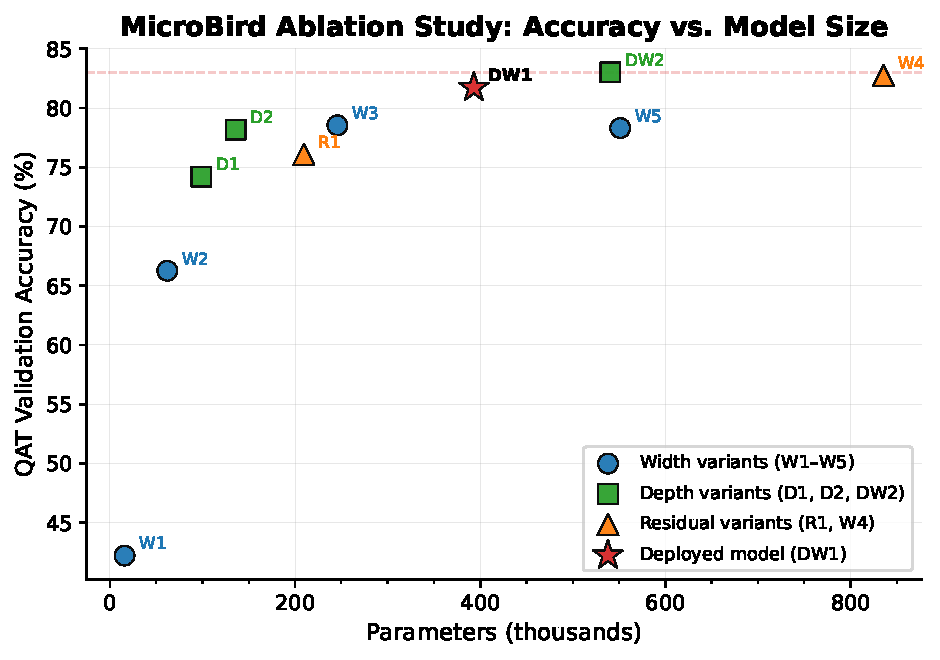
\includegraphics[width=\columnwidth]{fig4_ablation_scatter.pdf}
\caption{QAT validation accuracy vs.\ parameter count for all ten ablation configurations. DW1 and DW2 (stars) achieve the best accuracy--efficiency trade-off. W4 matches DW2 accuracy with 54\% more parameters and requires residual connections.}
\label{fig:ablation_scatter}
\end{figure}

The best-validated configuration is DW2 (32 channels, two extra depth blocks, no residual, 540,625 parameters, 83.01\% QAT validation accuracy). W3 (32 channels, no extra blocks, 245,695 parameters, 78.54\%) is the most compact model that still achieves strong accuracy and fits comfortably within the 512~KB CNN SRAM limit.

\subsection{Test Set Evaluation}
Configuration W3 was evaluated on the 3,034-sample held-out test set using the best QAT checkpoint, yielding 80.59\% top-1 and 91.53\% top-3 accuracy. The 10.94-percentage-point gap between top-1 and top-3 indicates that the correct class appears in the model's top three predictions in the large majority of error cases.

\begin{figure}[t]
\centering
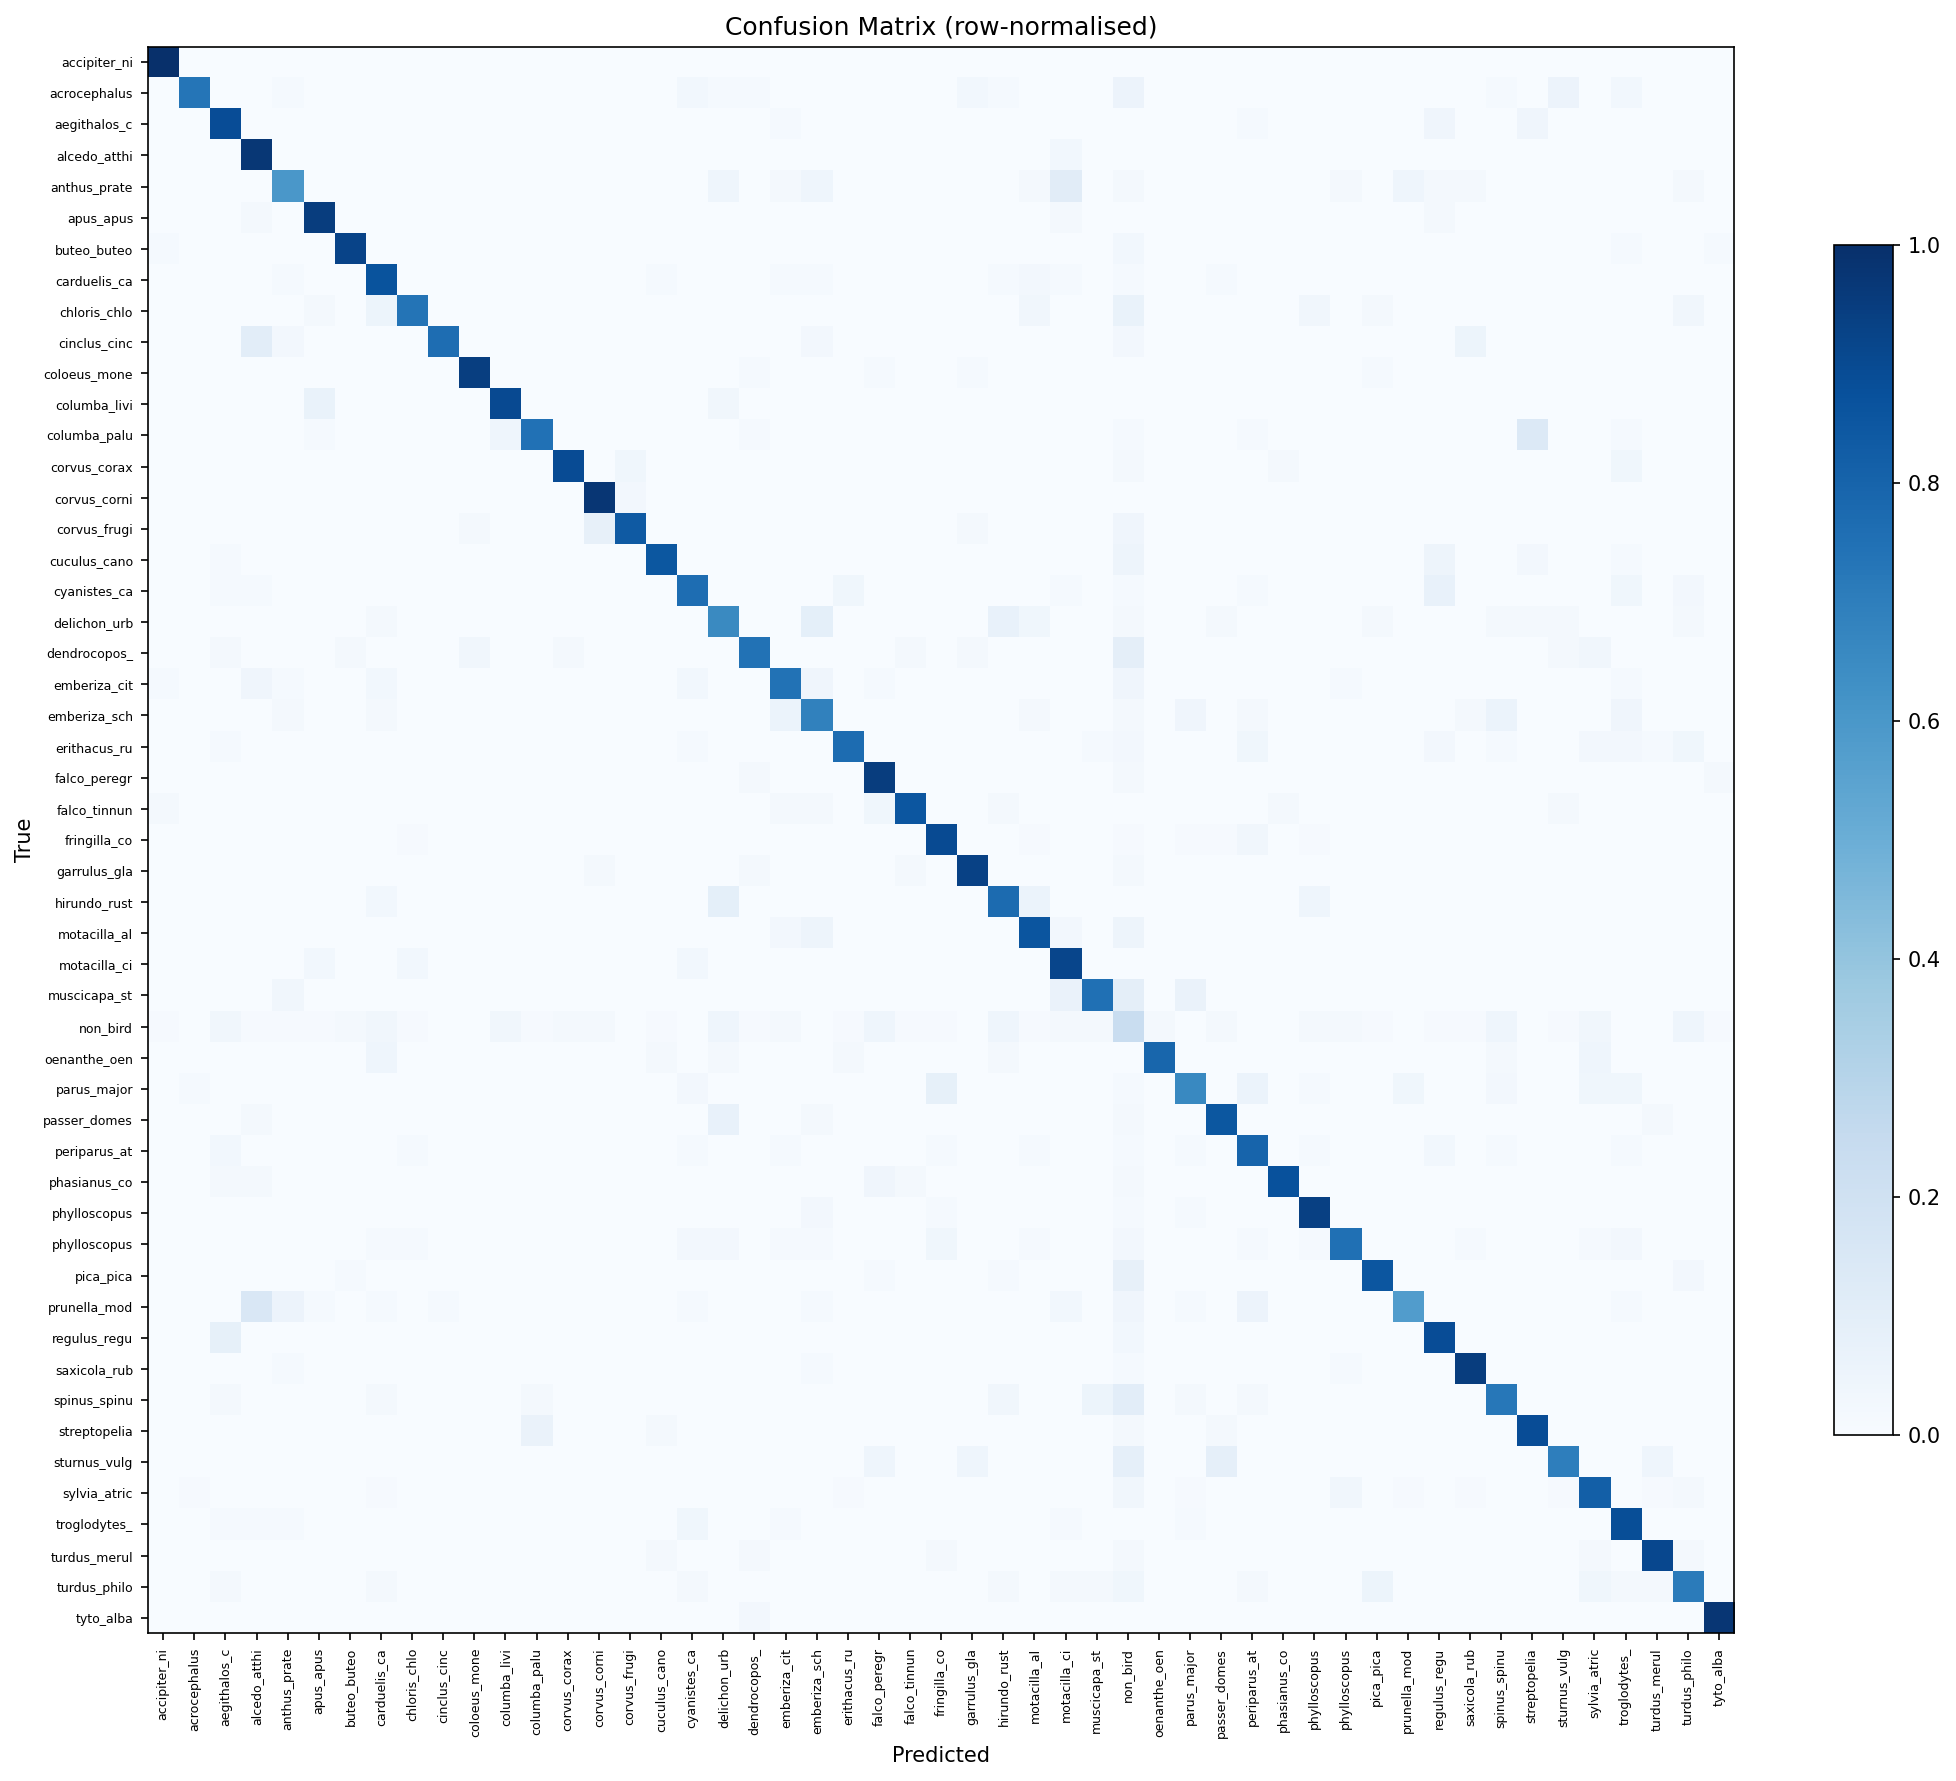
\includegraphics[width=\columnwidth]{fig5_confusion_matrix.png}
\caption{Row-normalised confusion matrix for W3 on the 3{,}034-sample held-out test set. The strong diagonal confirms most species are well-separated. The non-bird row (class 31) shows the primary weakness, with significant confusion across multiple bird species.}
\label{fig:confusion_matrix}
\end{figure}

\subsection{Per-Class Accuracy}
Table~\ref{tab:perclass} shows the five best and five worst per-class test accuracies for W3. The full breakdown across all 51 classes is provided in the Appendix.

\begin{table}[t]
\centering
\caption{Five best and five worst per-class test accuracies, W3 on test split.}
\label{tab:perclass}
\begin{tabular}{llrr}
\toprule
\textbf{Species} & \textbf{Common name} & \textbf{Acc.} & \textbf{$n$} \\
\midrule
\multicolumn{4}{l}{\textit{Best}} \\
\quad accipiter nisus      & Sparrowhawk    & 100.00\% & 23 \\
\quad corvus cornix        & Hooded Crow    &  97.44\% & 39 \\
\quad tyto alba            & Barn Owl       &  97.37\% & 38 \\
\quad falco peregrinus     & Peregrine      &  94.83\% & 58 \\
\quad coloeus monedula     & Jackdaw        &  94.52\% & 73 \\
\midrule
\multicolumn{4}{l}{\textit{Worst}} \\
\quad non\_bird            & Background     &  23.33\% & 90 \\
\quad prunella modularis   & Dunnock        &  57.53\% & 73 \\
\quad anthus pratensis     & Meadow Pipit   &  60.00\% & 45 \\
\quad delichon urbicum     & House Martin   &  65.45\% & 55 \\
\quad emberiza schoeniclus & Reed Bunting   &  68.63\% & 51 \\
\bottomrule
\end{tabular}
\end{table}

\begin{figure}[t]
\centering
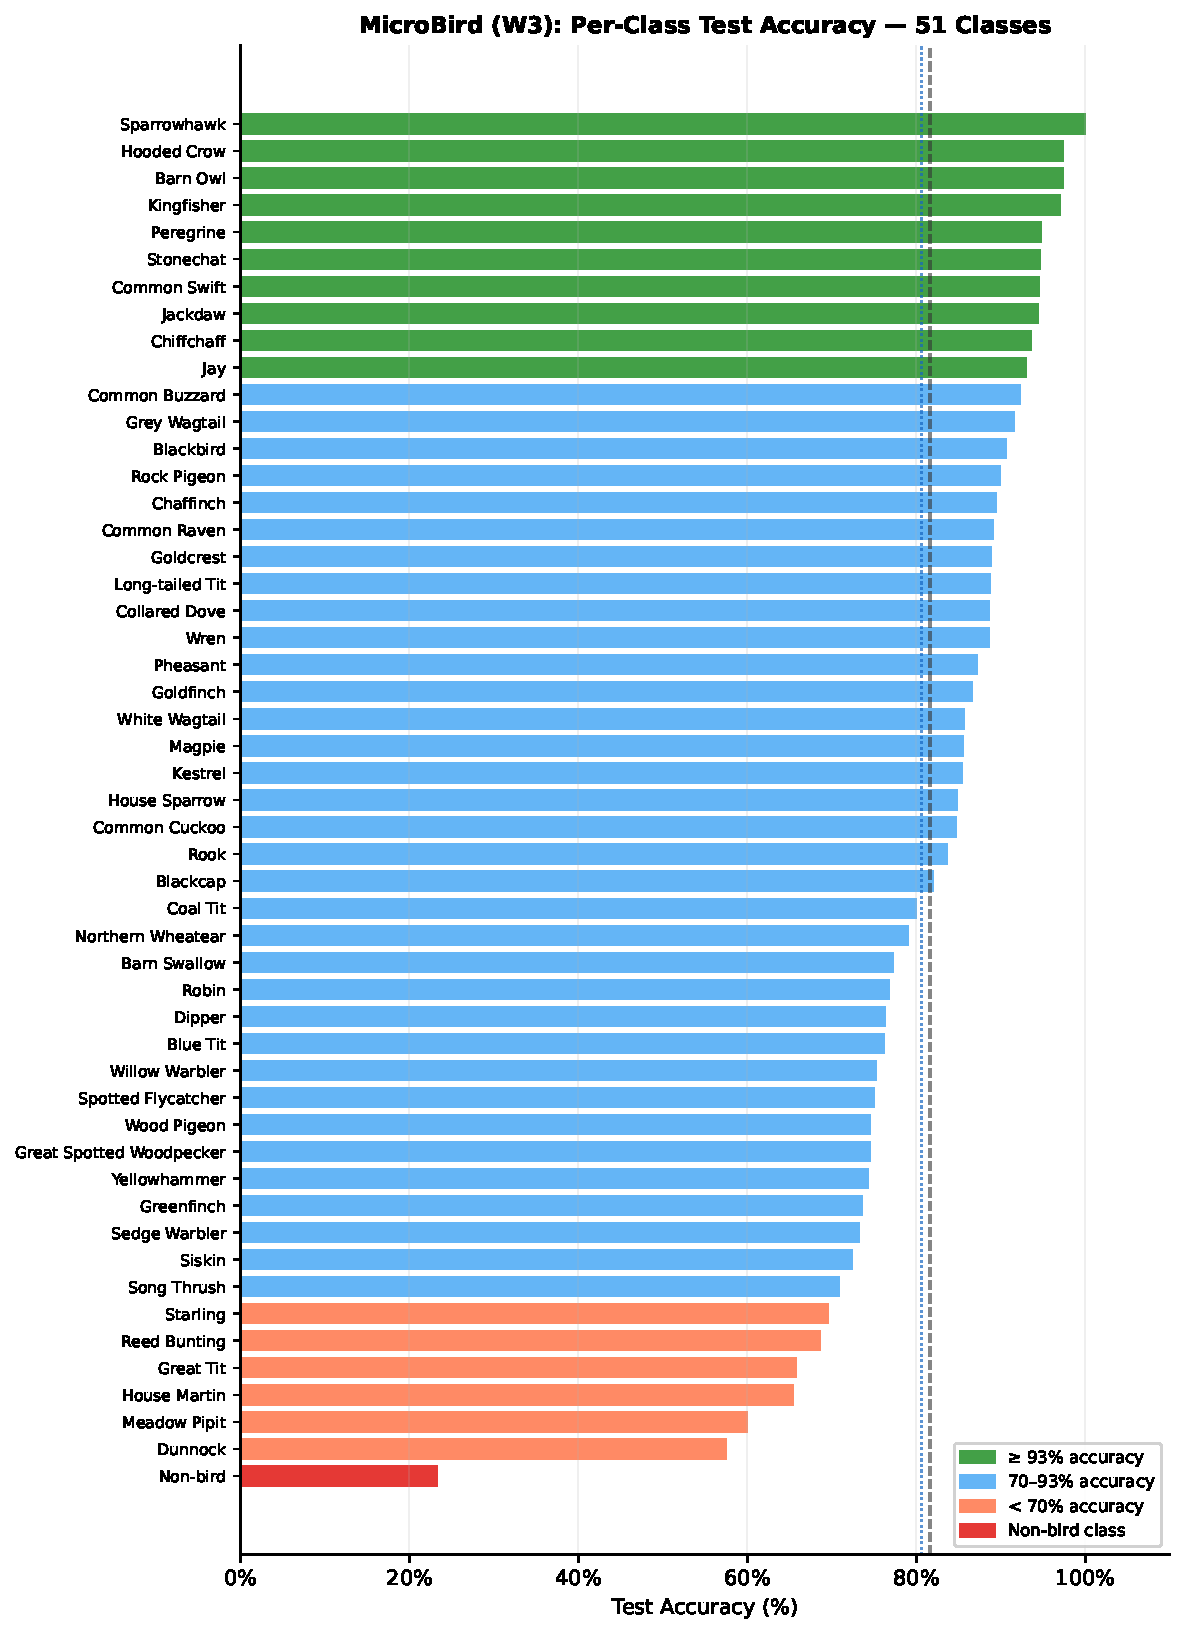
\includegraphics[width=\columnwidth]{fig6_perclass_accuracy.pdf}
\caption{Per-class test accuracy for W3, sorted ascending. The non-bird class (red) is the clear outlier at 23.3\%. Acoustically distinctive species (sparrowhawk, hooded crow, barn owl) reach near-perfect accuracy; thin-call species (dunnock, meadow pipit) are the weakest bird classes.}
\label{fig:perclass}
\end{figure}

\subsection{On-Device Performance}
The deployed model is DW1 (393,160 parameters, $\approx$384~KB weights), which fits within the 512~KB CNN SRAM limit and achieves 81.72\% QAT validation accuracy. End-to-end deployment evaluation was performed by replaying the full 3,034-sample held-out test split through the host inference API, which streams raw 3-second WAV clips to the board over UART and records returned predictions and timing metadata.

CNN inference time is measured using the \texttt{cnn\_time} hardware timer gating the CNN accelerator (MXC\_TMR1). Spectrogram computation time is measured using the ARM DWT cycle counter on the Cortex-M4. Table~\ref{tab:ondevice} summarises the measured values.

\begin{table}[t]
\centering
\caption{On-device inference timing and energy, DW1 on MAX78002 EvKit\_V1. CNN energy measured via hardware timer; spectrogram energy estimated from timing and M4 active-power figure ($\approx$10~mW at 80~MHz with FPU).}
\label{tab:ondevice}
\begin{tabular}{lrr}
\toprule
\textbf{Stage} & \textbf{Latency (ms)} & \textbf{Energy} \\
\midrule
CNN accelerator (200~MHz) & 3.5  & 15.3~\textmu J \\
Spectrogram -- Cortex-M4 (80~MHz) & 67.7 & $\approx$678~\textmu J \\
\midrule
Total per 3-second clip & 71.2 & $\approx$693~\textmu J \\
\bottomrule
\end{tabular}
\end{table}

The CNN accelerator completes inference in 3.5~ms and consumes 15.3~\textmu J, measured directly by the hardware timer. The Cortex-M4 spectrogram pipeline---comprising 184 overlapping RFFT windows, mel filterbank projection, per-sample normalisation, and int8 packing---requires 67.7~ms and accounts for approximately 98\% of total pipeline energy. The CNN accelerator therefore contributes only 2\% of the end-to-end energy budget despite performing the classification, demonstrating the efficiency advantage of dedicated hardware inference over general-purpose computation.

On the full 51-class deployed evaluation, DW1 achieves 79.10\% top-1 and 90.90\% top-3 accuracy across 3,034 held-out clips, with macro-$F_1=0.792$ and weighted-$F_1=0.789$. This end-to-end hardware/API result is only 1.49 percentage points below the offline W3 top-1 accuracy and 0.63 percentage points below its top-3 accuracy, indicating that the deployment pipeline preserves most of the accuracy of the best compact offline model while satisfying the MAX78002 memory budget. The dominant failure mode remains non-bird rejection rather than broad collapse across bird classes; by contrast, acoustically distinctive classes such as sparrowhawk, kingfisher, and buzzard retain recall above 96\% in deployed inference.

\subsection{Comparison with Baseline Models}
Table~\ref{tab:comparison} compares this work against three published embedded bird-call systems. BirdNET \cite{kahl2021birdnet} running on a Raspberry Pi 3B+ represents the current practical state of the art for edge deployment. TinyChirp \cite{huang2024tinychirp} targets binary single-species detection (Corn Bunting) on an nRF52840 Cortex-M4. WrenNet \cite{thoreau2025wrennet} performs 70-class alpine bird classification on an AudioMoth ($\leq$100~MHz, $\leq$1~MB RAM). All three report whole-board energy measured as supply current multiplied by inference time; no dedicated hardware timer isolates the neural network.

\begin{table}[t]
\centering
\caption{Comparison with published embedded bird audio systems. $\dagger$~Whole-board energy (general-purpose MCU, no accelerator). $\ddagger$~CNN accelerator only, measured via hardware timer; full pipeline $\approx$693~\textmu J.}
\label{tab:comparison}
\begin{tabular}{p{2cm}p{1.5cm}ccp{1.4cm}}
\toprule
\textbf{System} & \textbf{Platform} & \textbf{Classes} & \textbf{Top-1} & \textbf{Energy/clip} \\
\midrule
BirdNET \cite{kahl2021birdnet}     & RPi 3B+          & 3{,}000+ & ---   & 2{,}790~mJ$^\dagger$ \\
TinyChirp \cite{huang2024tinychirp} & nRF52840        & 1 (detect) & AUC $\approx$1.0 & 42.5~mJ$^\dagger$ \\
WrenNet \cite{thoreau2025wrennet}   & AudioMoth        & 70       & 70.1\% & 77~mJ$^\dagger$ \\
\midrule
\textbf{This work} (DW1) & \textbf{MAX78002} & \textbf{51} & \textbf{79.1\%} & \textbf{15.3~\textmu J}$^\ddagger$ \\
\bottomrule
\end{tabular}
\end{table}

On a whole-pipeline basis, this system consumes approximately 0.69~mJ per clip, which is 61$\times$ less than TinyChirp, 111$\times$ less than WrenNet, and over 4{,}000$\times$ less than BirdNET on a Raspberry Pi. These reductions are achieved while sustaining a 51-class task and higher top-1 accuracy than WrenNet (79.1\% vs.\ 70.1\%). The energy advantage is structural rather than incremental: a dedicated CNN accelerator completes inference at 15.3~\textmu J while the CPU-based systems spend tens of millijoules on the same step in software.

% =================================================================
\section{Analysis and Discussion}

\subsection{Width vs.\ Depth}
The ablation results reveal a consistent pattern: at fixed width, adding depth is a more parameter-efficient route to accuracy than increasing width alone. The D2 configuration (16 channels, 2 extra blocks, 135,697 parameters, 78.18\%) approaches the accuracy of W3 (32 channels, 0 extra blocks, 245,695 parameters, 78.54\%) while using 45\% fewer parameters. This is consistent with the literature showing that deeper networks extract more hierarchical spectral features \cite{sprengel2016audio}. The counter-intuitive result for W5 (48 channels, slightly lower accuracy than W3 at the same depth) reinforces this: increasing width without adding processing stages does not improve discriminative capacity.

\subsection{Effect of Residual Connections}
Comparing D2 (78.18\%) with R1 (76.09\%) shows that adding residual connections to the extra blocks decreases QAT accuracy while increasing parameter count. This is likely attributable to the \texttt{ai8x.Add()} operator imposing per-tensor activation range constraints that limit gradient flow through the shortcut path during QAT. The same effect holds at wider width: W4 (residual, 835,557 parameters, 82.75\%) trails DW2 (no residual, 540,625 parameters, 83.01\%) despite 54\% more parameters. Residual connections do not benefit this architecture at these scales.

\subsection{Quantization Impact}
Across most configurations, QAT accuracy equals or slightly exceeds float32 validation accuracy (e.g.\ W3: 78.08\% FP vs.\ 78.54\% QAT). This upward effect is consistent with published observations that quantization noise acts as a mild regulariser for small models \cite{jacob2018quantization}. The only configuration where QAT accuracy falls appreciably below FP is W1, where the model is so small that quantization noise is proportionally large relative to useful signal.

\subsection{The Non-Bird Class}
The non-bird class achieves only 23.33\% test accuracy, by far the lowest of all 51 classes. In the completed hardware/API replay, its precision is also only 29.6\%, confirming that this is a genuine class-definition weakness rather than a deployment-only regression. The non-bird class aggregates a highly diverse range of acoustic events---wind, rain, traffic, silence---whereas each bird species class is acoustically homogeneous. The model must learn to reject the full variety of non-biological sound with the same representational budget allocated to a single species' call. The teacher-filtering pipeline also collects non-bird clips by selecting the lowest-confidence BirdNET detections, which may introduce subtle acoustic ambiguity. Improving non-bird rejection is the highest-priority issue for future work.

\subsection{Per-Class Accuracy Patterns}
The completed deployed replay shows the same broad structure as the offline W3 analysis. Best-performing classes include sparrowhawk, kingfisher, buzzard, swift, and stonechat, all above 96\% recall; these species share acoustically distinctive calls with limited spectral overlap with any other class in the vocabulary. The weakest bird species after non-bird are dunnock, reed bunting, meadow pipit, and song thrush, which have thinner or less distinctive vocal structure and show stronger confusion with neighbouring passerine classes. Improved performance on these species would likely require a higher-resolution input or species-specific augmentation strategies.

\subsection{Energy and Efficiency}
The measured 15.3~\textmu J CNN inference energy places this system well within the regime targeted by dedicated AI microcontrollers. Published comparisons for the MAX78000---the predecessor chip---report 196--251~\textmu J for keyword-spotting pipelines on the same hardware class \cite{ulkar2021kws}, making the CNN-only result here 13--16$\times$ lower, reflecting the larger CNN SRAM and faster accelerator of the MAX78002 as well as the compact architecture chosen by the ablation study.

A notable implication of the energy breakdown is that the CNN accelerator is so efficient that scaling the class vocabulary has negligible energy cost. The output classifier layer for 120 classes instead of 50 adds fewer than 3~KB of weights; CNN inference energy would increase by less than 2~\textmu J while the spectrogram pipeline---the dominant cost at $\approx$678~\textmu J---remains unchanged. This is a property unavailable to software-only systems, where inference energy scales with model size.

For field deployment, the total per-clip energy of $\approx$0.69~mJ implies that a device performing continuous 3-second-window inference draws approximately 0.23~mW on average from the inference pipeline alone. A 1000~mAh, 3.7~V battery holds 3700~mWh; even accounting for microphone, UART, and idle M4 overheads, inference energy itself is not the limiting factor for deployment lifetime.

\subsection{Practical Deployment Trade-offs}
W3 (245,695 parameters, $\approx$240~KB at 8 bits) fits comfortably within the 512~KB CNN SRAM and has been fully validated through KAT on hardware. DW2 (540,625 parameters, $\approx$528~KB) exceeds the limit and requires explicit memory mapping before hardware confirmation. DW1 (393,160 parameters, $\approx$384~KB, 81.72\% QAT val) represents the best configuration that is both highly accurate and hardware-feasible; it is the validated deployment baseline used for the full 3,034-clip hardware/API evaluation.

% =================================================================
\section{Conclusion and Future Work}

This paper has presented MicroBird, a complete end-to-end pipeline for low-power embedded bird-call classification targeting Irish species monitoring on the MAX78002. Starting from raw community recordings, the pipeline produces a 30,201-sample, 51-class dataset via BirdNET teacher filtering, generates $64 \times 128$ log-mel spectrograms with per-sample normalisation, and trains a hardware-aware CNN using QAT. The model is synthesised and deployed to the MAX78002, where a matching on-device spectrogram pipeline enables inference without cloud connectivity. The system is demonstrated through a host-side API and web interface.

The ablation study establishes that 32 base channels is the optimal width for this task, depth blocks provide more accuracy per parameter than additional width, and residual connections offer no benefit after QAT. The best-validated model (DW2) achieves 83.01\% QAT validation accuracy; the offline W3 configuration reaches 80.59\% top-1 and 91.53\% top-3 on the held-out test set, while the deployed DW1 model reaches 79.10\% top-1 and 90.90\% top-3 when evaluated end-to-end through the hardware/API path on the same 3,034-sample split. The primary weakness is the non-bird background class at 23.33\% test accuracy.

On-device measurement confirms CNN inference energy of 15.3~\textmu J at 3.5~ms on the MAX78002 accelerator, with the Cortex-M4 spectrogram pipeline requiring 67.7~ms and dominating the 0.69~mJ total per clip. At this energy level, the inference pipeline itself consumes under 0.25~mW on a continuous 3-second-window schedule, making battery life a function of system idle power rather than inference cost.

Against published embedded bird classifiers, this system achieves 61--4{,}000$\times$ lower energy per clip while sustaining high 51-class accuracy and exceeding WrenNet's reported top-1 performance. The result demonstrates that dedicated CNN accelerators offer a qualitative rather than incremental efficiency advantage over general-purpose MCU deployment, and that MAX78002-class hardware is viable as the computational core of long-duration, battery-powered passive acoustic monitoring nodes.

Future work should address: deployment of higher-capacity variants such as DW2 if memory mapping can be resolved; a larger and more diverse non-bird corpus to improve background rejection; extended on-device evaluation with live microphone audio; and investigation of a sliding-window inference strategy for continuous monitoring rather than fixed 3-second clips.

\section*{Acknowledgment}
The author would like to thank Dr. Salaheddin Alakkari for his supervision and guidance throughout this project.

% =================================================================
\begin{thebibliography}{00}

\bibitem{kahl2021birdnet}
S. Kahl \textit{et al.}, ``BirdNET: A deep learning solution for avian diversity monitoring,'' \textit{Ecological Informatics}, vol. 61, 2021.

\bibitem{sprengel2016audio}
E. Sprengel, T. Jaggi, T. Kilcher, and T. Hofmann, ``Audio based bird species identification using deep learning techniques,'' in \textit{Working Notes of CLEF}, 2016.

\bibitem{park2019specaugment}
D. S. Park \textit{et al.}, ``SpecAugment: A simple data augmentation method for automatic speech recognition,'' in \textit{Proc. Interspeech}, 2019.

\bibitem{zhang2018mixup}
H. Zhang, M. Cisse, Y. N. Dauphin, and D. Lopez-Paz, ``mixup: Beyond empirical risk minimization,'' in \textit{Proc. ICLR}, 2018.

\bibitem{adi2022training}
Analog Devices, Inc., ``ai8x-training: Training and quantization for MAX78000/MAX78002,'' GitHub, 2022. [Online]. Available: \url{https://github.com/analogdevicesinc/ai8x-training}

\bibitem{jacob2018quantization}
B. Jacob \textit{et al.}, ``Quantization and training of neural networks for efficient integer-arithmetic-only inference,'' in \textit{Proc. CVPR}, 2018, pp. 2704--2713.

\bibitem{vellinga2015xc}
W. Vellinga and R. Planqu\'{e}, ``The Xeno-Canto collection and its relation to sound recognition and classification,'' in \textit{Proc. CLEF}, 2015.

\bibitem{warden2019tinyml}
P. Warden and D. Situnayake, \textit{TinyML: Machine Learning with TensorFlow Lite on Arduino and Ultra-Low-Power Microcontrollers}. O'Reilly Media, 2019.

\bibitem{huang2024tinychirp}
Z. Huang \textit{et al.}, ``TinyChirp: Bird song recognition using TinyML models on low-power wireless acoustic sensors,'' in \textit{Proc. IEEE Int. Symp. Internet of Sounds (IS2)}, Erlangen, Germany, Sep. 2024.

\bibitem{thoreau2025wrennet}
R. Thoreau \textit{et al.}, ``Enabling multi-species bird classification on low-power bioacoustic loggers,'' arXiv:2509.20103, 2025.

\bibitem{ulkar2021kws}
M. G. Ulkar and O. Okman, ``Ultra-low power keyword spotting at the edge,'' arXiv:2111.04988, 2021.

\end{thebibliography}

% =================================================================
\appendix
\section{Full Per-Class Test Accuracy (W3)}

\begin{table}[h]
\centering
\caption{Per-class test accuracy for W3 on the held-out test set (3,034 samples, 51 classes).}
\label{tab:full_perclass}
\small
\begin{tabular}{llrr}
\toprule
\textbf{Idx} & \textbf{Species} & \textbf{Acc.} & \textbf{$n$} \\
\midrule
0  & accipiter nisus            & 100.00\% & 23 \\
1  & acrocephalus schoenobaenus &  73.24\% & 71 \\
2  & aegithalos caudatus        &  88.73\% & 71 \\
3  & alcedo atthis              &  97.06\% & 34 \\
4  & anthus pratensis           &  60.00\% & 45 \\
5  & apus apus                  &  94.55\% & 55 \\
6  & buteo buteo                &  92.31\% & 65 \\
7  & carduelis carduelis        &  86.67\% & 75 \\
8  & chloris chloris            &  73.68\% & 57 \\
9  & cinclus cinclus            &  76.32\% & 38 \\
10 & coloeus monedula           &  94.52\% & 73 \\
11 & columba livia              &  90.00\% & 30 \\
12 & columba palumbus           &  74.63\% & 67 \\
13 & corvus corax               &  89.09\% & 55 \\
14 & corvus cornix              &  97.44\% & 39 \\
15 & corvus frugilegus          &  83.67\% & 49 \\
16 & cuculus canorus            &  84.81\% & 79 \\
17 & cyanistes caeruleus        &  76.25\% & 80 \\
18 & delichon urbicum           &  65.45\% & 55 \\
19 & dendrocopos major          &  74.60\% & 63 \\
20 & emberiza citrinella        &  74.29\% & 70 \\
21 & emberiza schoeniclus       &  68.63\% & 51 \\
22 & erithacus rubecula         &  76.83\% & 82 \\
23 & falco peregrinus           &  94.83\% & 58 \\
24 & falco tinnunculus          &  85.45\% & 55 \\
25 & fringilla coelebs          &  89.53\% & 86 \\
26 & garrulus glandarius        &  93.10\% & 58 \\
27 & hirundo rustica            &  77.27\% & 66 \\
28 & motacilla alba             &  85.71\% & 42 \\
29 & motacilla cinerea          &  91.67\% & 36 \\
30 & muscicapa striata          &  75.00\% & 32 \\
31 & non\_bird                  &  23.33\% & 90 \\
32 & oenanthe oenanthe          &  79.07\% & 43 \\
33 & parus major                &  65.85\% & 82 \\
34 & passer domesticus          &  84.91\% & 53 \\
35 & periparus ater             &  80.00\% & 70 \\
36 & phasianus colchicus        &  87.23\% & 47 \\
37 & phylloscopus collybita     &  93.67\% & 79 \\
38 & phylloscopus trochilus     &  75.31\% & 81 \\
39 & pica pica                  &  85.53\% & 76 \\
40 & prunella modularis         &  57.53\% & 73 \\
41 & regulus regulus            &  88.89\% & 36 \\
42 & saxicola rubicola          &  94.74\% & 76 \\
43 & spinus spinus              &  72.41\% & 58 \\
44 & streptopelia decaocto      &  88.71\% & 62 \\
45 & sturnus vulgaris           &  69.57\% & 23 \\
46 & sylvia atricapilla         &  82.02\% & 89 \\
47 & troglodytes troglodytes    &  88.61\% & 79 \\
48 & turdus merula              &  90.62\% & 64 \\
49 & turdus philomelos          &  70.91\% & 55 \\
50 & tyto alba                  &  97.37\% & 38 \\
\midrule
   & \textbf{Overall (top-1)}   & \textbf{80.59\%} & 3034 \\
\bottomrule
\end{tabular}
\end{table}

\end{document}
